\documentclass[12pt,a4paper]{article}

\usepackage[utf8]{inputenc}
\usepackage[T1]{fontenc}
\usepackage{geometry}
\usepackage{graphicx}
\usepackage{listings}
\usepackage{xcolor}
\usepackage{hyperref}
\usepackage{amsmath}
\usepackage{amssymb}
\usepackage{booktabs}
\usepackage{float}
\usepackage{subcaption}
\usepackage{tikz}
\usepackage{pgfplots}

\geometry{
    left=2.5cm,
    right=2.5cm,
    top=2.5cm,
    bottom=2.5cm
}

% Define colors for code listings
\definecolor{codegreen}{rgb}{0,0.6,0}
\definecolor{codegray}{rgb}{0.5,0.5,0.5}
\definecolor{codepurple}{rgb}{0.58,0,0.82}
\definecolor{backcolour}{rgb}{0.95,0.95,0.95}

% Python code listing configuration
\lstdefinestyle{pystyle}{
    backgroundcolor=\color{backcolour},
    commentstyle=\color{codegreen},
    keywordstyle=\color{magenta},
    numberstyle=\tiny\color{codegray},
    stringstyle=\color{codepurple},
    basicstyle=\ttfamily\footnotesize,
    breakatwhitespace=false,
    breaklines=true,
    captionpos=b,
    keepspaces=true,
    numbers=left,
    numbersep=5pt,
    showspaces=false,
    showstringspaces=false,
    showtabs=false,
    tabsize=4
}

\lstset{style=pystyle}

\title{OpenRadioss Workbench for FreeCAD: \\ LS-DYNA Workflow Documentation}
\author{OpenRadioss Development Team}
\date{\today}

\begin{document}

\maketitle

\begin{abstract}
This document provides comprehensive documentation for the OpenRadioss workbench, a FreeCAD extension that enables seamless creation and management of LS-DYNA input files (.k files). The workbench provides an integrated environment for finite element analysis preprocessing, combining FreeCAD's powerful 3D modeling capabilities with LS-DYNA's simulation power.
\end{abstract}

\tableofcontents

\newpage

\section{Introduction}

\subsection{Overview}
The OpenRadioss workbench is a specialized FreeCAD extension designed to bridge the gap between 3D modeling and finite element analysis. It provides tools for creating, editing, and exporting LS-DYNA input files directly within the FreeCAD environment.

\subsection{Motivation}
Traditional finite element analysis workflows require multiple software tools:
\begin{itemize}
    \item CAD software for geometry creation
    \item Preprocessing software for meshing and analysis setup
    \item Solver input file generation
    \item Post-processing and visualization
\end{itemize}

The OpenRadioss workbench consolidates these steps by providing an integrated solution within FreeCAD.

\subsection{Key Features}
\begin{itemize}
    \item Interactive LS-DYNA keyword editor with parameter management
    \item Template-based .k file generation with predefined structures
    \item Text-based document objects for .k file storage and editing
    \item Export functionality for generating production-ready .k files
    \item Persistent storage in FreeCAD's native .FCStd format
\end{itemize}

\section{Architecture and Design}

\subsection{Organizational Structure}
The OpenRadioss workbench follows a hierarchical structure that organizes functionality into logical layers. The following organizational chart provides a visual representation of the system architecture:

\newpage
\begin{figure}[H]
    \centering
    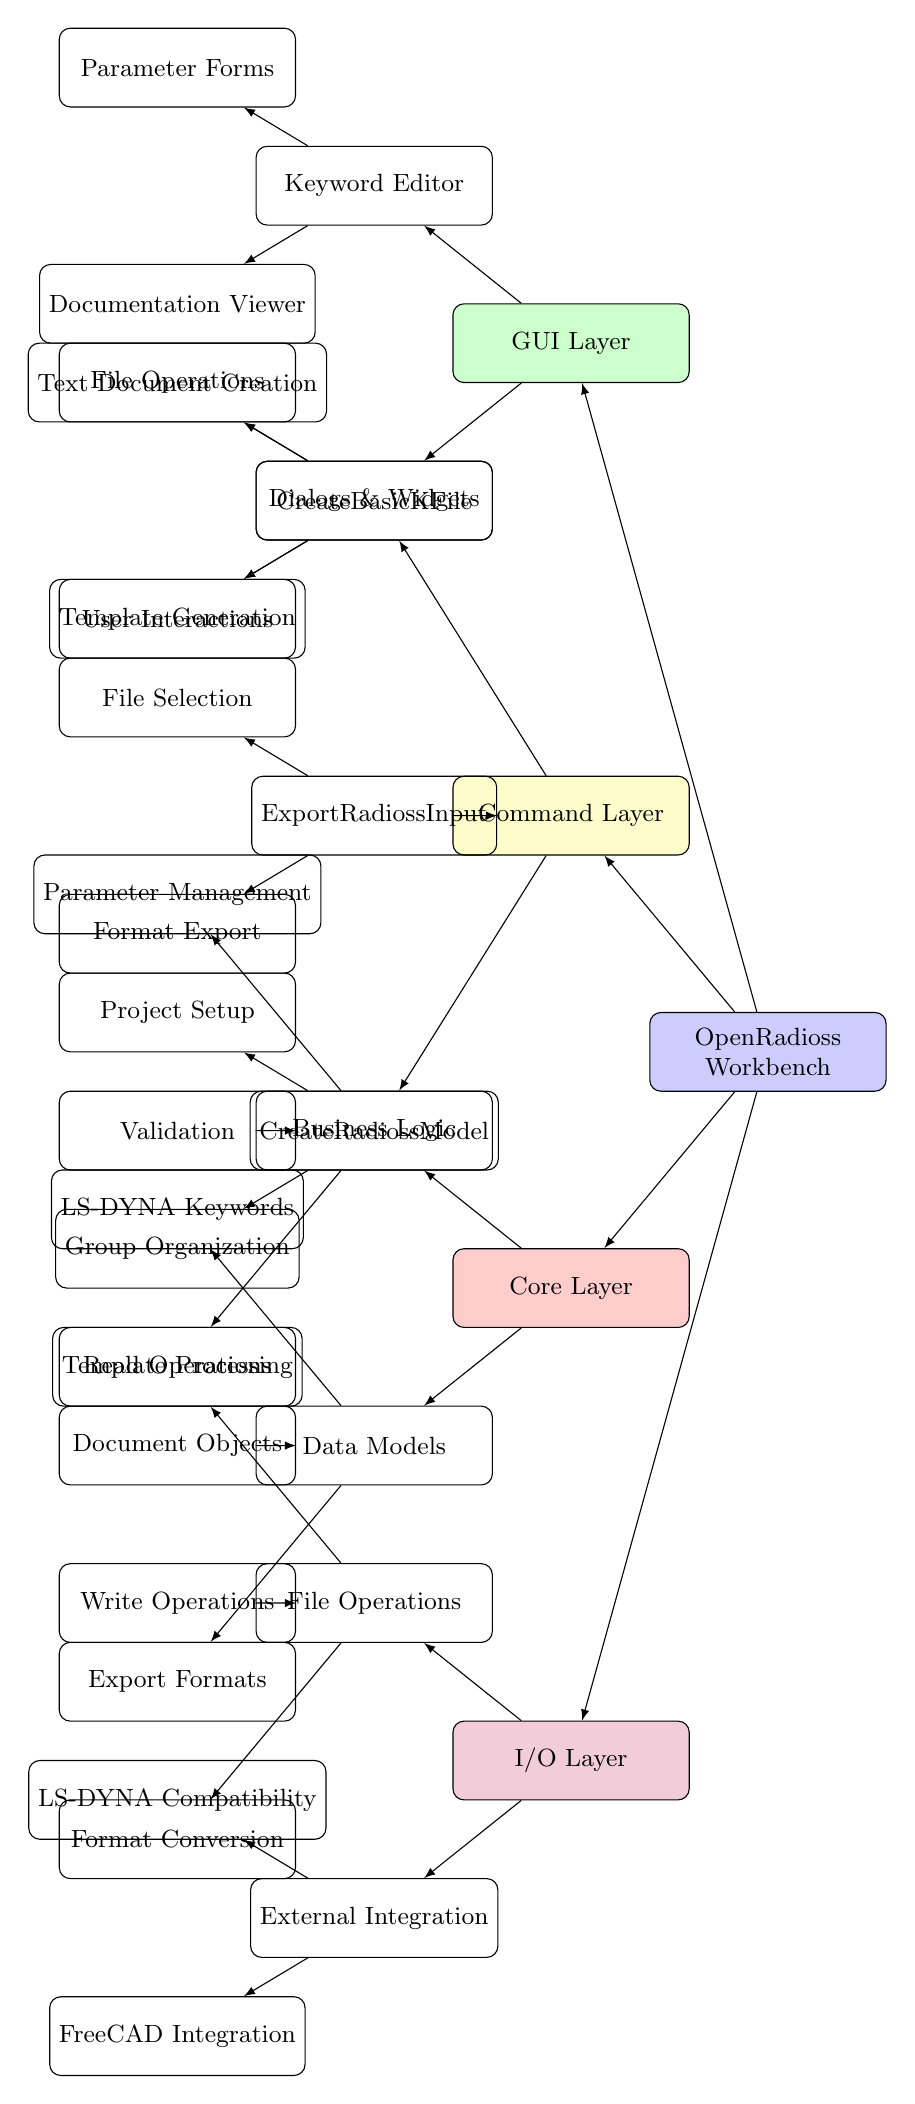
\begin{tikzpicture}[
        level distance=2.5cm,
        level 1/.style={sibling distance=6cm},
        level 2/.style={sibling distance=4cm},
        level 3/.style={sibling distance=3cm},
        every node/.style={draw, rectangle, rounded corners, minimum width=3cm, minimum height=1cm, align=center, font=\small},
        edge from parent/.style={draw, -latex},
        rotate=-90  % Rotate 90 degrees counter-clockwise
    ]

    % Root node
    \node[fill=blue!20] {OpenRadioss\\Workbench}
        child { node[fill=green!20] {GUI Layer}
            child { node {Keyword Editor}
                child { node {Parameter Forms} }
                child { node {Documentation Viewer} }
            }
            child { node {Dialogs \& Widgets}
                child { node {File Operations} }
                child { node {User Interactions} }
            }
        }
        child { node[fill=yellow!20] {Command Layer}
            child { node {CreateBasicKFile}
                child { node {Text Document Creation} }
                child { node {Template Generation} }
            }
            child { node {ExportRadiossInput}
                child { node {File Selection} }
                child { node {Format Export} }
            }
            child { node {CreateRadiossModel}
                child { node {Project Setup} }
                child { node {Group Organization} }
            }
        }
        child { node[fill=red!20] {Core Layer}
            child { node {Business Logic}
                child { node {Parameter Management} }
                child { node {Validation} }
                child { node {Template Processing} }
            }
            child { node {Data Models}
                child { node {LS-DYNA Keywords} }
                child { node {Document Objects} }
                child { node {Export Formats} }
            }
        }
        child { node[fill=purple!20] {I/O Layer}
            child { node {File Operations}
                child { node {Read Operations} }
                child { node {Write Operations} }
                child { node {Format Conversion} }
            }
            child { node {External Integration}
                child { node {LS-DYNA Compatibility} }
                child { node {FreeCAD Integration} }
            }
        };

    \end{tikzpicture}
    \caption{OpenRadioss Workbench Organizational Structure (Rotated 90° CCW)}
    \label{fig:organigram}
\end{figure}

\clearpage
\subsection{Architecture Layer Details}
This section provides detailed explanations of each architectural layer shown in the organizational chart.

\subsection{Component Structure}

\subsubsection{GUI Components}
\begin{itemize}
    \item \texttt{KeywordEditorDialog}: Main interface for keyword parameter editing
    \item \texttt{DocumentationViewer}: Integrated help and documentation system
    \item Custom dialogs for file operations and user interactions
\end{itemize}

\subsubsection{Command Components}
\begin{itemize}
    \item \texttt{CreateBasicKFile}: Creates LS-DYNA text document objects
    \item \texttt{ExportRadiossInput}: Exports .k files from text documents
    \item \texttt{CreateRadiossModel}: Initializes new analysis projects
\end{itemize}

\subsubsection{Core Logic}
\begin{itemize}
    \item Parameter parsing and validation
    \item LS-DYNA keyword template management
    \item Text document object management
    \item Export formatting and validation
\end{itemize}

\section{User Workflow}

\subsection{Getting Started}

\subsubsection{Installation}
The OpenRadioss workbench is installed as a standard FreeCAD workbench:

\begin{enumerate}
    \item Copy the workbench directory to FreeCAD's Mod directory
    \item Restart FreeCAD
    \item Activate the workbench from the workbench selector
\end{enumerate}

\subsubsection{Initial Setup}
\begin{enumerate}
    \item Launch FreeCAD
    \item Select "OpenRadioss" from the workbench dropdown
    \item The workbench toolbar and menus will be available
\end{enumerate}

\subsection{Creating LS-DYNA Files}

\subsubsection{Step 1: Create Basic Template}
Click "Create Basic .k File" to generate a new LS-DYNA text document:

\begin{lstlisting}[language=Python, caption=Creating LS-DYNA text document]
# Creates App::TextDocument object with LS-DYNA content
k_file_obj = doc.addObject("App::TextDocument", "LSDynaKeywords")
k_file_obj.Text = generate_basic_k_file_content()
\end{lstlisting}

The generated template includes:
\begin{itemize}
    \item Control cards (termination, timestep, output)
    \item Database output definitions
    \item Material and section definitions
    \item Sample geometry (nodes and elements)
\end{itemize}

\subsubsection{Step 2: Edit Content}
The .k file content can be edited in several ways:

\begin{enumerate}
    \item \textbf{Property Panel}: Select the object and edit the "Text" property
    \item \textbf{Export and Edit}: Export to .k file, edit externally, then re-import
    \item \textbf{Keyword Editor}: Use the advanced keyword editor for parameter management
\end{enumerate}

\subsubsection{Step 3: Export to .k File}
Click "Export LS-DYNA .k File" to generate the final .k file:

\begin{lstlisting}[language=Python, caption=Export functionality]
# Find TextDocument objects
for obj in App.ActiveDocument.Objects:
    if obj.TypeId == 'App::TextDocument' and obj.Text:
        # Export obj.Text to .k file
        with open(filepath, 'w') as f:
            f.write(obj.Text)
\end{lstlisting}

\subsection{Advanced Workflow}

\subsubsection{Using the Keyword Editor}
The keyword editor provides advanced parameter management:

\begin{enumerate}
    \item Select keywords from categorized lists
    \item Configure parameters through GUI forms
    \item Generate keyword text with parameter substitution
    \item Preview and validate before export
\end{enumerate}

\subsubsection{Project Organization}
\begin{itemize}
    \item Create separate FreeCAD documents for different analyses
    \item Use document groups to organize related objects
    \item Maintain version control through FreeCAD's document system
\end{itemize}

\section{Technical Implementation}

\subsection{Text Document Management}

\subsubsection{Creating Text Documents}
\begin{lstlisting}[language=Python, caption=Text document creation]
def create_k_file_document(self):
    """Create LS-DYNA text document in FreeCAD."""
    doc = App.ActiveDocument or App.newDocument("LSDyna_Model")

    # Create TextDocument object
    k_file_obj = doc.addObject("App::TextDocument", "LSDynaKeywords")
    k_file_obj.Label = "LS-DYNA Keywords"
    k_file_obj.Text = self._generate_basic_k_file_content()

    return k_file_obj
\end{lstlisting}

\subsubsection{Content Structure}
The .k file content follows LS-DYNA format specifications:

\begin{itemize}
    \item \texttt{*KEYWORD}: File header
    \item \texttt{*CONTROL\_*}: Simulation control parameters
    \item \texttt{*DATABASE\_*}: Output specification
    \item \texttt{*PART}: Part definitions
    \item \texttt{*SECTION\_*}: Section properties
    \item \texttt{*MAT\_*}: Material definitions
    \item \texttt{*NODE}: Nodal coordinates
    \item \texttt{*ELEMENT\_*}: Element connectivity
    \item \texttt{*END}: File termination
\end{itemize}

\subsection{Export System}

\subsubsection{Export Process}
\begin{enumerate}
    \item Identify TextDocument objects in active document
    \item Extract text content from objects
    \item Present selection dialog if multiple objects exist
    \item Write content to .k file with proper formatting
    \item Open file in external editor if available
\end{enumerate}

\subsubsection{Error Handling}
\begin{lstlisting}[language=Python, caption=Export error handling]
try:
    # Export logic
    success = export_k_file(selected_obj, filepath)
    if success:
        show_success_message(filepath)
except Exception as e:
    show_error_message(f"Export failed: {str(e)}")
\end{lstlisting}

\subsection{GUI Integration}

\subsubsection{Workbench Registration}
\begin{lstlisting}[language=Python, caption=Workbench initialization]
class OpenRadiossWorkbench(Workbench):
    def Initialize(self):
        # Import and register commands
        from .commands.create_basic_k_file import CreateBasicKFile
        from .commands.export_radioss_input import ExportRadiossInput

        Gui.addCommand('CreateBasicKFile', CreateBasicKFile())
        Gui.addCommand('ExportRadiossInput', ExportRadiossInput())

        # Create toolbar and menu
        self.appendToolbar("OpenRadioss", [
            "CreateBasicKFile", "ExportRadiossInput"
        ])
\end{lstlisting}

\subsubsection{Command Pattern}
Each workbench command follows the standard FreeCAD command pattern:

\begin{lstlisting}[language=Python, caption=Command class structure]
class ExampleCommand:
    def GetResources(self):
        return {
            'Pixmap': 'icon_path',
            'MenuText': 'Command Name',
            'ToolTip': 'Description'
        }

    def Activated(self):
        # Command implementation
        pass

    def IsActive(self):
        # Availability check
        return True
\end{lstlisting}

\section{LS-DYNA Template Structure}

\subsection{Control Cards}
\begin{lstlisting}[language=Python, caption=Control card generation]
*CONTROL_TERMINATION
$  endtim    endcyc     dtmin       endeng     endmas
     1.0
$
*CONTROL_TIMESTEP
$  dtinit    scft     isdo     tsd0       dt2ms       dtmp       dt2ms
     0.0     0.0     0.0     0.0
\end{lstlisting}

\subsection{Database Output}
\begin{lstlisting}[language=Python, caption=Database output configuration]
*DATABASE_BINARY_D3PLOT
$  dt/cycl  lcdt      ioopt
   0.01
$
*DATABASE_GLSTAT
$  dt/cycl  lcdt      ioopt
   0.01
\end{lstlisting}

\subsection{Material and Section Definitions}
\begin{lstlisting}[language=Python, caption=Material definitions]
*PART
$      pid     secid       mid     eosid      hgid      grav    adpopt
         1         1         1         0         0         0         0
$
*SECTION_SHELL
$     sid    elform      shrf       nip     propt   qr/irid     icomp    setyp
        1         2     1.000     3.000         0         0         0         0
$
*MAT_ELASTIC
$      mid        ro         e        pr         da         db         k
         1    7.8e-9     2.0e5      0.30
\end{lstlisting}

\subsection{Geometry Definitions}
\begin{lstlisting}[language=Python, caption=Sample geometry]
*NODE
$     nid               x               y               z      tc      rc
         1       0.000000       0.000000       0.000000       0       0
         2       1.000000       0.000000       0.000000       0       0
         3       1.000000       1.000000       0.000000       0       0
         4       0.000000       1.000000       0.000000       0       0
$
*ELEMENT_SHELL
$     eid     pid      n1      n2      n3      n4
         1       1       1       2       3       4
\end{lstlisting}

\section{File Format and Persistence}

\subsection{FreeCAD Document Storage}
The LS-DYNA content is stored as TextDocument objects within FreeCAD's native .FCStd format:

\begin{itemize}
    \item Document objects persist across FreeCAD sessions
    \item Content is stored in compressed binary format
    \item Version control compatible through FreeCAD's document system
    \item Automatic backup and recovery support
\end{itemize}

\subsection{Export Format}
The .k file export maintains exact LS-DYNA formatting:

\begin{itemize}
    \item Proper keyword ordering and structure
    \item Correct column alignment for numerical data
    \item Comment preservation
    \item LS-DYNA compatibility verification
\end{itemize}

\section{Integration with LS-DYNA}

\subsection{Compatibility}
The generated .k files are compatible with:
\begin{itemize}
    \item LS-DYNA R7 and later versions
    \item Standard LS-DYNA ASCII input format
    \item Common LS-DYNA keywords and parameters
\end{itemize}

\subsection{Best Practices}
\begin{enumerate}
    \item Validate generated .k files before production use
    \item Use appropriate units (consistent unit system)
    \item Verify material properties and boundary conditions
    \item Test with simple models before complex analyses
\end{enumerate}

\section{Development and Extension}

\subsection{Code Organization}
\begin{lstlisting}[language=bash, caption=Project structure]
freecad/ORfemn/
├── __init__.py           # Main workbench class
├── init_gui.py           # GUI initialization
├── gui/                  # GUI components
│   └── keyword_editor.py # Advanced keyword editor
├── commands/             # Command implementations
│   ├── create_basic_k_file.py
│   ├── export_radioss_input.py
│   └── create_radioss_model.py
└── docs/                 # Documentation
\end{lstlisting}

\subsection{Adding New Keywords}
To add support for new LS-DYNA keywords:

\begin{enumerate}
    \item Update the keywords JSON database
    \item Add parameter definitions and validation
    \item Implement GUI forms for parameter input
    \item Add export formatting logic
\end{enumerate}

\subsection{Customization}
The workbench can be customized by:
\begin{itemize}
    \item Modifying template content in \texttt{\_generate\_basic\_k\_file\_content()}
    \item Adding new command classes for specialized workflows
    \item Extending the keyword database with domain-specific keywords
\end{itemize}

\section{Troubleshooting}

\subsection{Common Issues}

\subsubsection{Export Failures}
\begin{itemize}
    \item Check file permissions and disk space
    \item Verify TextDocument object exists and has content
    \item Ensure proper file path specification
\end{itemize}

\subsubsection{GUI Issues}
\begin{itemize}
    \item Restart FreeCAD if workbench doesn't load
    \item Check Python path and module imports
    \item Verify Qt/PySide installation compatibility
\end{itemize}

\subsection{Debug Information}
Enable debug logging by setting:
\begin{lstlisting}[language=Python]
import logging
logging.basicConfig(level=logging.DEBUG)
\end{lstlisting}

\section{Conclusion}

The OpenRadioss workbench provides a powerful and intuitive solution for LS-DYNA preprocessing within FreeCAD. By combining the strengths of both platforms, it offers a streamlined workflow from 3D modeling to finite element analysis.

\subsection{Future Enhancements}
\begin{itemize}
    \item Advanced meshing integration
    \item Post-processing result visualization
    \item Multi-physics coupling support
    \item Cloud-based collaboration features
\end{itemize}

\subsection{Contributing}
Contributions are welcome through:
\begin{itemize}
    \item Bug reports and feature requests
    \item Code contributions and improvements
    \item Documentation enhancements
    \item Test case development
\end{itemize}

\end{document}
